% Options for packages loaded elsewhere
\PassOptionsToPackage{unicode}{hyperref}
\PassOptionsToPackage{hyphens}{url}
\PassOptionsToPackage{dvipsnames,svgnames,x11names}{xcolor}
%
\documentclass[
  letterpaper,
  DIV=11,
  numbers=noendperiod]{scrartcl}

\usepackage{amsmath,amssymb}
\usepackage{iftex}
\ifPDFTeX
  \usepackage[T1]{fontenc}
  \usepackage[utf8]{inputenc}
  \usepackage{textcomp} % provide euro and other symbols
\else % if luatex or xetex
  \usepackage{unicode-math}
  \defaultfontfeatures{Scale=MatchLowercase}
  \defaultfontfeatures[\rmfamily]{Ligatures=TeX,Scale=1}
\fi
\usepackage{lmodern}
\ifPDFTeX\else  
    % xetex/luatex font selection
\fi
% Use upquote if available, for straight quotes in verbatim environments
\IfFileExists{upquote.sty}{\usepackage{upquote}}{}
\IfFileExists{microtype.sty}{% use microtype if available
  \usepackage[]{microtype}
  \UseMicrotypeSet[protrusion]{basicmath} % disable protrusion for tt fonts
}{}
\makeatletter
\@ifundefined{KOMAClassName}{% if non-KOMA class
  \IfFileExists{parskip.sty}{%
    \usepackage{parskip}
  }{% else
    \setlength{\parindent}{0pt}
    \setlength{\parskip}{6pt plus 2pt minus 1pt}}
}{% if KOMA class
  \KOMAoptions{parskip=half}}
\makeatother
\usepackage{xcolor}
\setlength{\emergencystretch}{3em} % prevent overfull lines
\setcounter{secnumdepth}{-\maxdimen} % remove section numbering
% Make \paragraph and \subparagraph free-standing
\makeatletter
\ifx\paragraph\undefined\else
  \let\oldparagraph\paragraph
  \renewcommand{\paragraph}{
    \@ifstar
      \xxxParagraphStar
      \xxxParagraphNoStar
  }
  \newcommand{\xxxParagraphStar}[1]{\oldparagraph*{#1}\mbox{}}
  \newcommand{\xxxParagraphNoStar}[1]{\oldparagraph{#1}\mbox{}}
\fi
\ifx\subparagraph\undefined\else
  \let\oldsubparagraph\subparagraph
  \renewcommand{\subparagraph}{
    \@ifstar
      \xxxSubParagraphStar
      \xxxSubParagraphNoStar
  }
  \newcommand{\xxxSubParagraphStar}[1]{\oldsubparagraph*{#1}\mbox{}}
  \newcommand{\xxxSubParagraphNoStar}[1]{\oldsubparagraph{#1}\mbox{}}
\fi
\makeatother

\usepackage{color}
\usepackage{fancyvrb}
\newcommand{\VerbBar}{|}
\newcommand{\VERB}{\Verb[commandchars=\\\{\}]}
\DefineVerbatimEnvironment{Highlighting}{Verbatim}{commandchars=\\\{\}}
% Add ',fontsize=\small' for more characters per line
\usepackage{framed}
\definecolor{shadecolor}{RGB}{241,243,245}
\newenvironment{Shaded}{\begin{snugshade}}{\end{snugshade}}
\newcommand{\AlertTok}[1]{\textcolor[rgb]{0.68,0.00,0.00}{#1}}
\newcommand{\AnnotationTok}[1]{\textcolor[rgb]{0.37,0.37,0.37}{#1}}
\newcommand{\AttributeTok}[1]{\textcolor[rgb]{0.40,0.45,0.13}{#1}}
\newcommand{\BaseNTok}[1]{\textcolor[rgb]{0.68,0.00,0.00}{#1}}
\newcommand{\BuiltInTok}[1]{\textcolor[rgb]{0.00,0.23,0.31}{#1}}
\newcommand{\CharTok}[1]{\textcolor[rgb]{0.13,0.47,0.30}{#1}}
\newcommand{\CommentTok}[1]{\textcolor[rgb]{0.37,0.37,0.37}{#1}}
\newcommand{\CommentVarTok}[1]{\textcolor[rgb]{0.37,0.37,0.37}{\textit{#1}}}
\newcommand{\ConstantTok}[1]{\textcolor[rgb]{0.56,0.35,0.01}{#1}}
\newcommand{\ControlFlowTok}[1]{\textcolor[rgb]{0.00,0.23,0.31}{\textbf{#1}}}
\newcommand{\DataTypeTok}[1]{\textcolor[rgb]{0.68,0.00,0.00}{#1}}
\newcommand{\DecValTok}[1]{\textcolor[rgb]{0.68,0.00,0.00}{#1}}
\newcommand{\DocumentationTok}[1]{\textcolor[rgb]{0.37,0.37,0.37}{\textit{#1}}}
\newcommand{\ErrorTok}[1]{\textcolor[rgb]{0.68,0.00,0.00}{#1}}
\newcommand{\ExtensionTok}[1]{\textcolor[rgb]{0.00,0.23,0.31}{#1}}
\newcommand{\FloatTok}[1]{\textcolor[rgb]{0.68,0.00,0.00}{#1}}
\newcommand{\FunctionTok}[1]{\textcolor[rgb]{0.28,0.35,0.67}{#1}}
\newcommand{\ImportTok}[1]{\textcolor[rgb]{0.00,0.46,0.62}{#1}}
\newcommand{\InformationTok}[1]{\textcolor[rgb]{0.37,0.37,0.37}{#1}}
\newcommand{\KeywordTok}[1]{\textcolor[rgb]{0.00,0.23,0.31}{\textbf{#1}}}
\newcommand{\NormalTok}[1]{\textcolor[rgb]{0.00,0.23,0.31}{#1}}
\newcommand{\OperatorTok}[1]{\textcolor[rgb]{0.37,0.37,0.37}{#1}}
\newcommand{\OtherTok}[1]{\textcolor[rgb]{0.00,0.23,0.31}{#1}}
\newcommand{\PreprocessorTok}[1]{\textcolor[rgb]{0.68,0.00,0.00}{#1}}
\newcommand{\RegionMarkerTok}[1]{\textcolor[rgb]{0.00,0.23,0.31}{#1}}
\newcommand{\SpecialCharTok}[1]{\textcolor[rgb]{0.37,0.37,0.37}{#1}}
\newcommand{\SpecialStringTok}[1]{\textcolor[rgb]{0.13,0.47,0.30}{#1}}
\newcommand{\StringTok}[1]{\textcolor[rgb]{0.13,0.47,0.30}{#1}}
\newcommand{\VariableTok}[1]{\textcolor[rgb]{0.07,0.07,0.07}{#1}}
\newcommand{\VerbatimStringTok}[1]{\textcolor[rgb]{0.13,0.47,0.30}{#1}}
\newcommand{\WarningTok}[1]{\textcolor[rgb]{0.37,0.37,0.37}{\textit{#1}}}

\providecommand{\tightlist}{%
  \setlength{\itemsep}{0pt}\setlength{\parskip}{0pt}}\usepackage{longtable,booktabs,array}
\usepackage{calc} % for calculating minipage widths
% Correct order of tables after \paragraph or \subparagraph
\usepackage{etoolbox}
\makeatletter
\patchcmd\longtable{\par}{\if@noskipsec\mbox{}\fi\par}{}{}
\makeatother
% Allow footnotes in longtable head/foot
\IfFileExists{footnotehyper.sty}{\usepackage{footnotehyper}}{\usepackage{footnote}}
\makesavenoteenv{longtable}
\usepackage{graphicx}
\makeatletter
\def\maxwidth{\ifdim\Gin@nat@width>\linewidth\linewidth\else\Gin@nat@width\fi}
\def\maxheight{\ifdim\Gin@nat@height>\textheight\textheight\else\Gin@nat@height\fi}
\makeatother
% Scale images if necessary, so that they will not overflow the page
% margins by default, and it is still possible to overwrite the defaults
% using explicit options in \includegraphics[width, height, ...]{}
\setkeys{Gin}{width=\maxwidth,height=\maxheight,keepaspectratio}
% Set default figure placement to htbp
\makeatletter
\def\fps@figure{htbp}
\makeatother

\KOMAoption{captions}{tableheading}
\makeatletter
\@ifpackageloaded{caption}{}{\usepackage{caption}}
\AtBeginDocument{%
\ifdefined\contentsname
  \renewcommand*\contentsname{Table of contents}
\else
  \newcommand\contentsname{Table of contents}
\fi
\ifdefined\listfigurename
  \renewcommand*\listfigurename{List of Figures}
\else
  \newcommand\listfigurename{List of Figures}
\fi
\ifdefined\listtablename
  \renewcommand*\listtablename{List of Tables}
\else
  \newcommand\listtablename{List of Tables}
\fi
\ifdefined\figurename
  \renewcommand*\figurename{Figure}
\else
  \newcommand\figurename{Figure}
\fi
\ifdefined\tablename
  \renewcommand*\tablename{Table}
\else
  \newcommand\tablename{Table}
\fi
}
\@ifpackageloaded{float}{}{\usepackage{float}}
\floatstyle{ruled}
\@ifundefined{c@chapter}{\newfloat{codelisting}{h}{lop}}{\newfloat{codelisting}{h}{lop}[chapter]}
\floatname{codelisting}{Listing}
\newcommand*\listoflistings{\listof{codelisting}{List of Listings}}
\makeatother
\makeatletter
\makeatother
\makeatletter
\@ifpackageloaded{caption}{}{\usepackage{caption}}
\@ifpackageloaded{subcaption}{}{\usepackage{subcaption}}
\makeatother

\ifLuaTeX
  \usepackage{selnolig}  % disable illegal ligatures
\fi
\usepackage{bookmark}

\IfFileExists{xurl.sty}{\usepackage{xurl}}{} % add URL line breaks if available
\urlstyle{same} % disable monospaced font for URLs
\hypersetup{
  pdftitle={Tutorial 1: automated stratigraphic correlation using StratoBayes},
  colorlinks=true,
  linkcolor={blue},
  filecolor={Maroon},
  citecolor={Blue},
  urlcolor={Blue},
  pdfcreator={LaTeX via pandoc}}


\title{Tutorial 1: automated stratigraphic correlation using
StratoBayes}
\author{}
\date{}

\begin{document}
\maketitle


\begin{quote}
For more information on StratoBayes, or to install the software, please
visit \url{https://stratobayes.github.io/}. Resources
\end{quote}

The goal of this tutorial is to take stratigraphic data from two
sections and shift and stretch or squeeze one section relative to the
other, to align them:

\begin{figure}

\begin{minipage}{0.48\linewidth}

\begin{figure}[H]

\centering{

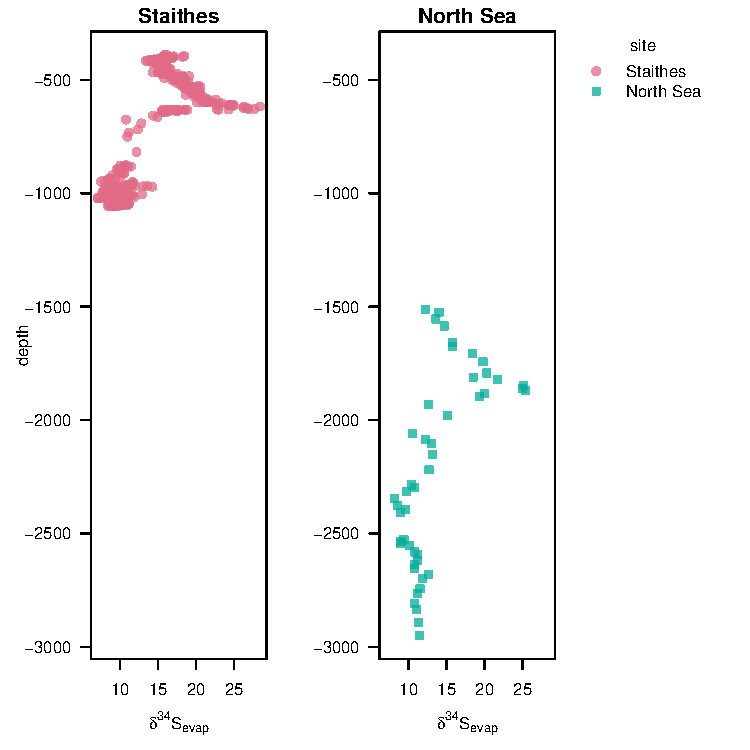
\includegraphics{StratoBayes-Tutorial-1_files/figure-pdf/fig-3-1.pdf}

}

\caption{\label{fig-3-1}Sulphur isotope data from two sites on their
original depth scale.}

\end{figure}%

\end{minipage}%
%
\begin{minipage}{0.04\linewidth}
~\end{minipage}%
%
\begin{minipage}{0.48\linewidth}

\begin{figure}[H]

\centering{

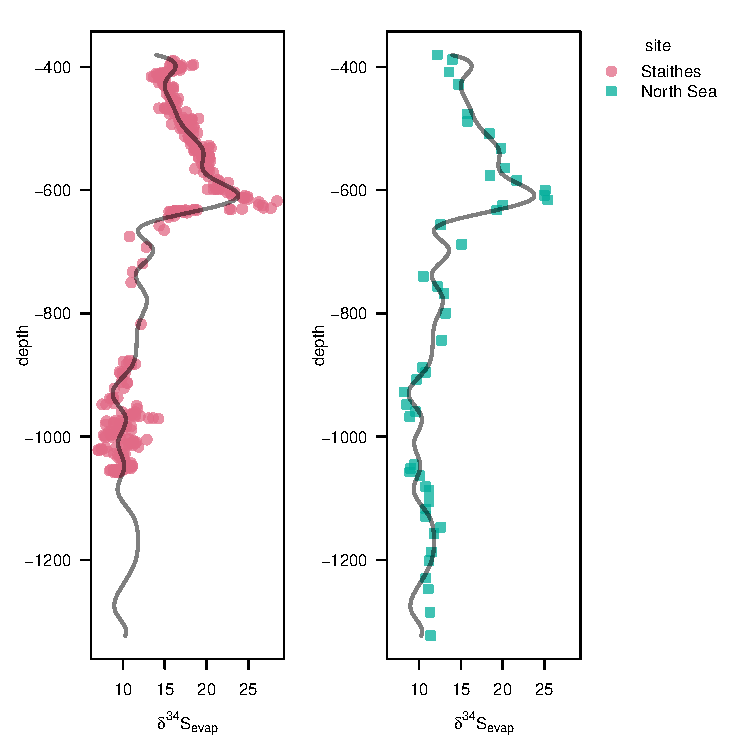
\includegraphics{StratoBayes-Tutorial-1_files/figure-pdf/fig-3-2.pdf}

}

\caption{\label{fig-3-2}North Sea data has been shifted and squeezed to
align with the Staithes data.}

\end{figure}%

\end{minipage}%

\end{figure}%

In the figure above, the depths associated with the sulphur isotope data
from a North Sea well (blue) have been transformed to match the data
from the Staithes well (red).

Below is a step-by-step guide to correlate the two wells using the
\texttt{StratoBayes} R package, starting with an introduction to the
data sets involved.

\section{Permian -- Triassic sulphur isotope
data}\label{permian-triassic-sulphur-isotope-data}

The Permian-Triassic strata of the United Kingdom are difficult to date
due to a scarcity of biostratigraphic constraints. Salisbury et
al.~(2023) have used sulphur isotope ratios from evaporites
(\(\delta^{34}S_{evap}\)) to correlate a a well from the southern North
Sea Basin (42/28-2) with a drillcore from Staithes (Cleveland Basin,
Yorkshire, UK). The \(\delta^{34}S_{evap}\) of evaporites is assumed to
reflect the ceoval isotopic composition of seawater.

\begin{figure}[H]

\centering{

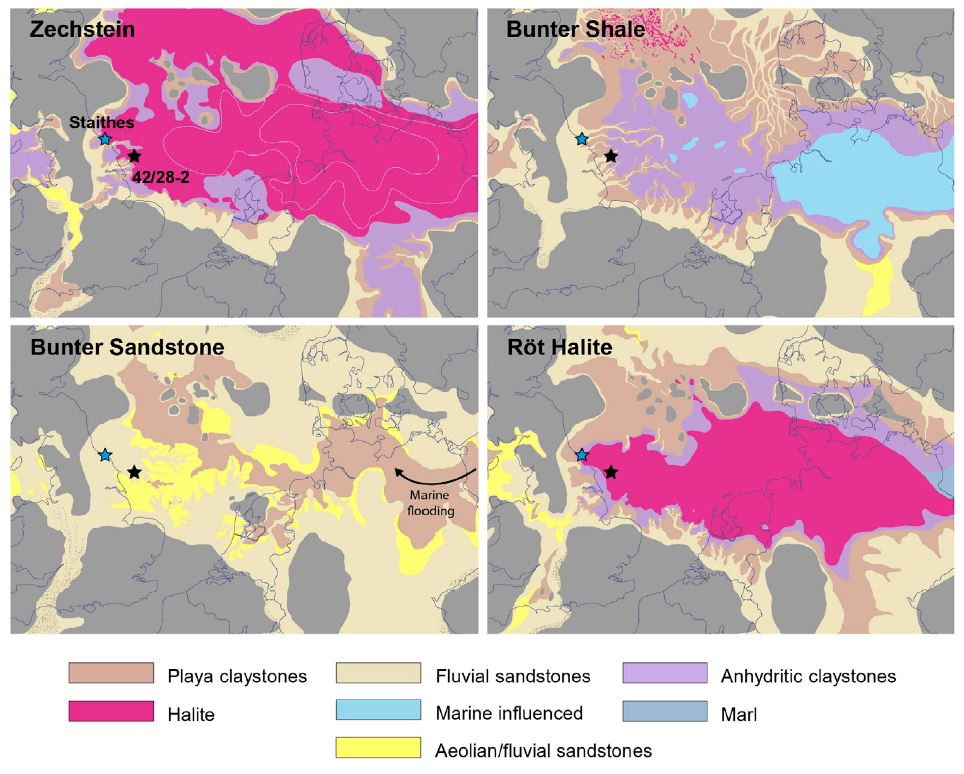
\includegraphics{images/Salisbury2023-fig1.jpg}

}

\caption{\label{fig-1}Palaeogeographic context of the two wells,
Salisbury et al.~(2023)}

\end{figure}%

The authors correlated the two curves by visually matching several peaks
and troughs of the \(\delta^{34}S_{evap}\) curves:

\begin{figure}[H]

\centering{

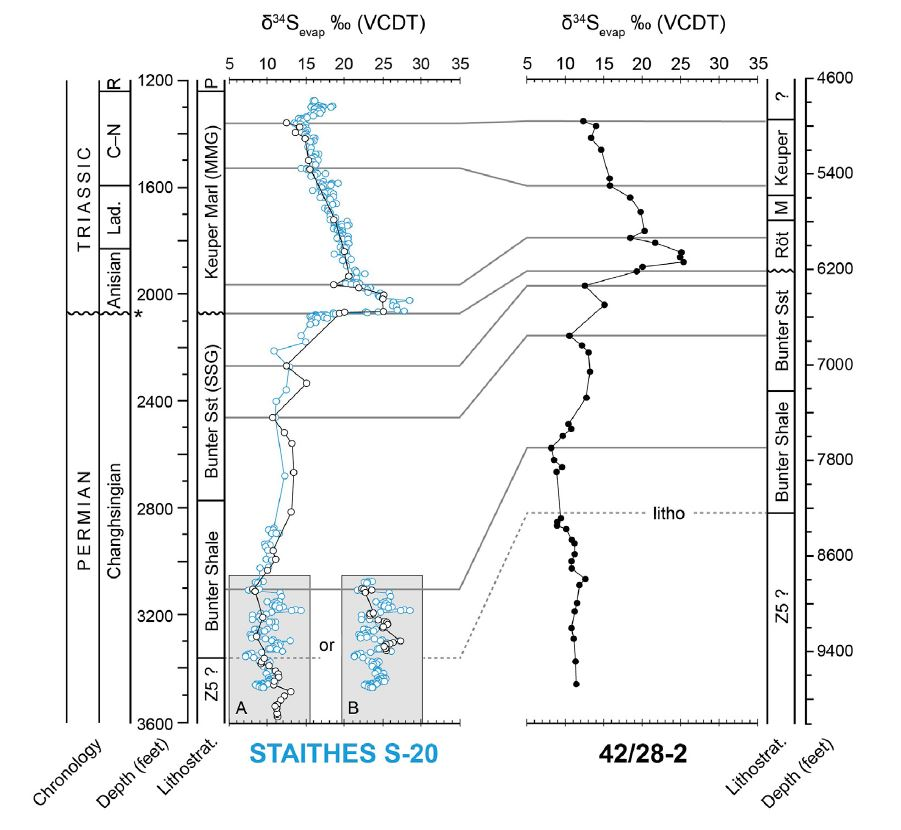
\includegraphics{images/Salisbury2023-fig4.jpg}

}

\caption{\label{fig-2}Correlation of \(\delta^{34}S_{evap}\) from the
two wells, Salisbury et al.~(2023)}

\end{figure}%

We will now try to recreate that correlation using StratoBayes.

\section{Preparing the data}\label{preparing-the-data}

We have downloaded the data from the North Sea well from the
Supplementary Materials of
\href{https://doi.org/10.3389/feart.2023.1216365}{Salisbury et
al.~(2023)}, and received the data from Staithes from the authors of
\href{https://doi.org/10.1038/s41598-022-21542-4}{Salisbury et
al.~(2022)}. These data were saved as .xlsx files. To facilitate reading
the data in R, we copied the relevant data (depth and
\(\delta^{34}S_{evap}\) measurements) into new Excel spreadsheets with
clean column names, and saved them as .csv files.

For reading the files, we first check what our working directory is:

\begin{Shaded}
\begin{Highlighting}[]
\FunctionTok{getwd}\NormalTok{()}
\end{Highlighting}
\end{Shaded}

\begin{verbatim}
[1] "D:/Github/stratobayes.github.io/tutorial-1"
\end{verbatim}

If you are running the code chunks in the
\texttt{StratoBayes1\_Correlation.qmd} file, your working directory will
be wherever that file is saved. Otherwise, if you are running the code
from a regular R script, you can set your desired working directory
using \texttt{setwd}.

Assuming the data sets are in a folder named ``data'' in your working
directory, we can start reading the data with R:

\begin{Shaded}
\begin{Highlighting}[]
\CommentTok{\# set random seed to ensure consistency of results}
\FunctionTok{set.seed}\NormalTok{(}\DecValTok{1}\NormalTok{)}
\CommentTok{\# read the .csv files}
\NormalTok{north\_sea }\OtherTok{\textless{}{-}} \FunctionTok{read.csv}\NormalTok{(}\StringTok{"data/North\_Sea{-}d34S.csv"}\NormalTok{)}
\NormalTok{staithes }\OtherTok{\textless{}{-}} \FunctionTok{read.csv}\NormalTok{(}\StringTok{"data/Staithes{-}S20{-}d34S.csv"}\NormalTok{)}
\CommentTok{\# display the beginning of the data.frames}
\FunctionTok{head}\NormalTok{(north\_sea)}
\end{Highlighting}
\end{Shaded}

\begin{verbatim}
  depth d34S
1  4960 12.2
2  5000 14.0
3  5100 13.6
4  5200 14.7
5  5440 15.8
6  5500 15.8
\end{verbatim}

\begin{Shaded}
\begin{Highlighting}[]
\FunctionTok{head}\NormalTok{(staithes)}
\end{Highlighting}
\end{Shaded}

\begin{verbatim}
    depth  d34S
1 1280.17 15.86
2 1280.67 16.13
3 1300.00 18.44
4 1300.17 15.72
5 1303.00 17.05
6 1303.92 15.60
\end{verbatim}

The StratoBayes package expects all chemostratigraphic data to be in a
single spreadsheet or data.frame. We can achieve this by combining the
two data.frames:

\begin{Shaded}
\begin{Highlighting}[]
\CommentTok{\# add site identifiers:}
\NormalTok{north\_sea}\SpecialCharTok{$}\NormalTok{site }\OtherTok{\textless{}{-}} \StringTok{"North Sea"}
\NormalTok{staithes}\SpecialCharTok{$}\NormalTok{site }\OtherTok{\textless{}{-}} \StringTok{"Staithes"}
\CommentTok{\# combine data.frames}
\NormalTok{dataset }\OtherTok{\textless{}{-}} \FunctionTok{rbind}\NormalTok{(north\_sea, staithes)}
\CommentTok{\# transform depth measurements from feet to m}
\NormalTok{dataset}\SpecialCharTok{$}\NormalTok{depth }\OtherTok{\textless{}{-}}\NormalTok{ dataset}\SpecialCharTok{$}\NormalTok{depth }\SpecialCharTok{*} \FloatTok{0.3048}
\CommentTok{\# check n data points per site:}
\FunctionTok{table}\NormalTok{(dataset}\SpecialCharTok{$}\NormalTok{site)}
\end{Highlighting}
\end{Shaded}

\begin{verbatim}

North Sea  Staithes 
       47       364 
\end{verbatim}

\section{The StratoBayes workflow}\label{the-stratobayes-workflow}

\subsection{Reading data with
StratoBayes}\label{reading-data-with-stratobayes}

Now we can process this data with the StratoBayes package. First, we
need to load the package:

\begin{Shaded}
\begin{Highlighting}[]
\CommentTok{\# load the StratoBayes library}
\FunctionTok{library}\NormalTok{(}\StringTok{"StratoBayes"}\NormalTok{)}
\end{Highlighting}
\end{Shaded}

We start by reading it with the \texttt{StratData()} function. We
specify ``d34S'' as the name of the column holding our stratigraphic
signal. As the Staithes section has a lot more data than the North Sea
section, we specify ``Staithes'' as our reference site. Because the data
are organized along depth -- representing the vertical (or ``z'')
stratigraphic dimension -- and this information is stored in the
``depth'' column, we set both \texttt{zScale} and \texttt{zColumn} to
``depth''.

\begin{Shaded}
\begin{Highlighting}[]
\CommentTok{\# read data with the StratData function}
\NormalTok{stratDat }\OtherTok{\textless{}{-}} \FunctionTok{StratData}\NormalTok{(}\AttributeTok{signal =}\NormalTok{ dataset, }\AttributeTok{signalColumn =} \StringTok{"d34S"}\NormalTok{, }
                      \AttributeTok{referenceSite =} \StringTok{"Staithes"}\NormalTok{, }
                      \AttributeTok{zScale =} \StringTok{"depth"}\NormalTok{, }\AttributeTok{zColumn =} \StringTok{"depth"}\NormalTok{)}
\CommentTok{\# check the class of this object}
\FunctionTok{class}\NormalTok{(stratDat)}
\end{Highlighting}
\end{Shaded}

\begin{verbatim}
[1] "StratData" "list"     
\end{verbatim}

\texttt{stratDat} is now an object of class ``StratData''. The
\texttt{print()} function will recognise this and print some information
on the dataset:

\begin{Shaded}
\begin{Highlighting}[]
\CommentTok{\# this is equivalent to print(stratDat) or print.StratData(stratDat)}
\NormalTok{stratDat}
\end{Highlighting}
\end{Shaded}

\begin{verbatim}
Stratigraphic data comprising 1 signal from 2 sites
\end{verbatim}

The \texttt{plot()} function visualises the signal data from both sites:

\begin{Shaded}
\begin{Highlighting}[]
\CommentTok{\# visualise stratDat using plot.StratData(stratDat)}
\FunctionTok{plot}\NormalTok{(stratDat)}
\end{Highlighting}
\end{Shaded}

\begin{figure}[H]

\centering{

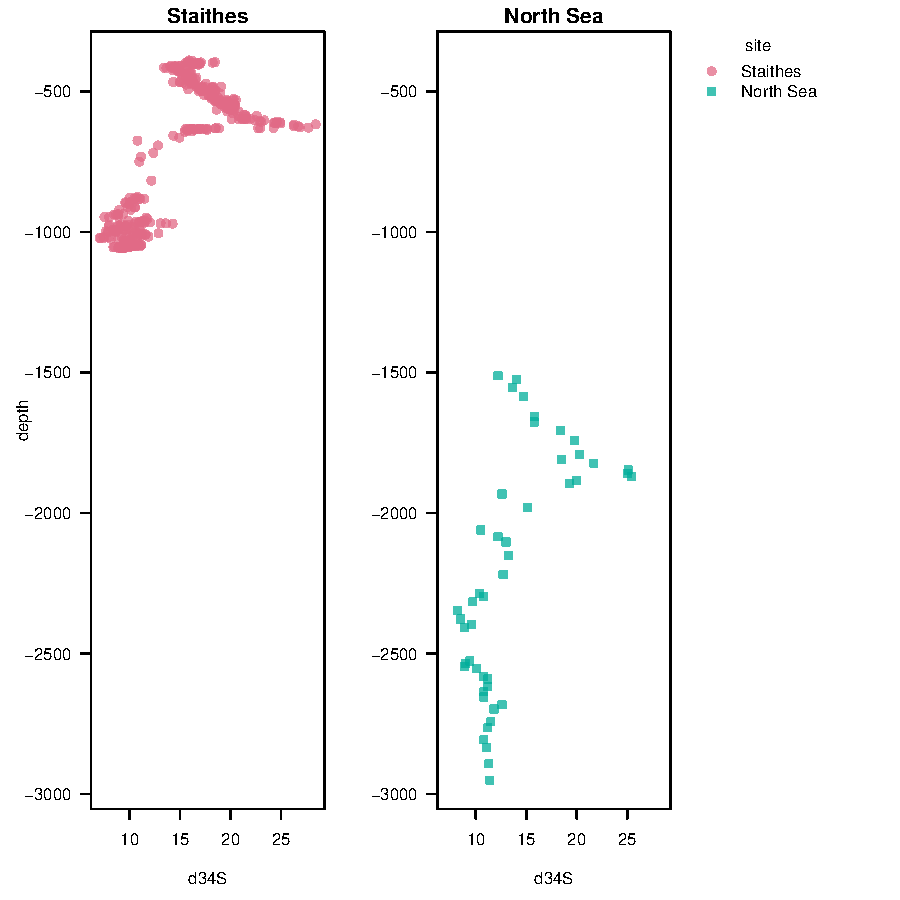
\includegraphics{StratoBayes-Tutorial-1_files/figure-pdf/fig-5-1.pdf}

}

\caption{\label{fig-5}Sulphur isotope data from the Staithes and the
North Sea well}

\end{figure}%

\emph{Notice that depths have been internally multiplied by -1 to allow
for calculations as if measurements were on the height scale, and for
easier plotting.}

\subsection{Building a stratigraphic
model}\label{building-a-stratigraphic-model}

We can now think about how we want to align the two sections. A simple
option would be to shift the North Sea section and apply a ``stretch''
factor that compresses the section to match the Staithes section. The
Staithes section is thus our reference section and remains unchanged. We
need a single ``stretch'' factor or sedimentation rate (\(\gamma\)) for
the aligned section, as well as an offset or shift that corresponds to
the depth in the reference section to which the bottom of the aligned
section will be shifted (\(\alpha\)).

Calculating the depth at the reference site (Staithes) that corresponds
to a depth at the North Sea site is done as follows:
\[depth_{Staithes} = \alpha + \gamma * \Delta_{North Sea}~,\]\\
where \(\Delta_{North Sea}\) is the distance from the bottom of the
North Sea section to the depth of interest.

\emph{Note that depths are internally multiplied by -1 to allow for
calculations as if measurements were on the height scale, and for easier
plotting}.

\subsection{The Bayesian framework}\label{the-bayesian-framework}

How do we find the \(\alpha\) and \(\gamma\) that lead to the best
alignment?

StratoBayes estimates those parameters in the Bayesian framework by

\begin{itemize}
\item
  placing priors on \(\alpha\) and \(\gamma\)
\item
  defining a likelihood based on the deviations of the sulphur isotope
  data from a cubic spline fitted to the (depth-shifted) sulphur isotope
  data from both sites
\item
  running a Markov-chain Monte Carlo (MCMC) simulation to find the
  posterior distribution of \(\alpha\) and \(\gamma\)
\end{itemize}

\subsection{Priors}\label{priors}

We will need to place priors on the shift and the stretch factor. To
find out what the priors need to look like, we use the
\texttt{StratModelTemplate()} function. We specify that the sections
will be aligned on a height or depth scale (alignmentScale =
``height''), rather than on an age scale. We further specify that our
sedimentation rate model has one rate per site (sedModel = ``site'').

\begin{Shaded}
\begin{Highlighting}[]
\CommentTok{\# get a template for the priors}
\FunctionTok{StratModelTemplate}\NormalTok{(}\AttributeTok{stratData =}\NormalTok{ stratDat, }\AttributeTok{alignmentScale =} \StringTok{"height"}\NormalTok{, }\AttributeTok{sedModel =} \StringTok{"site"}\NormalTok{)}
\end{Highlighting}
\end{Shaded}

\begin{verbatim}

priors <- structure(list(
  "alpha_North Sea" = UniformPrior(min = , max = ),
  "gammaLog_North Sea" = NormalPrior(mean = , sd = )),
  class = c("StratPrior", "list"))

model <- StratModel(stratData = stratDat,
                    priors = priors,
                    alignmentScale = "height",
                    sedModel = "site",
                    alphaPosition = "middle",
                    nKnots = 25)

result <- RunStratModel(stratObject = stratDat,
                        stratModel = model,
                        nRun = 1,
                        nIter = 1000)
\end{verbatim}

\begin{verbatim}
`stratData` consists of depth-scale measurements. To facilitate data processing, depths have been converted to heights by multiplying them by `-1`. Please use negative depths (i.e. heights) to specify the priors on `alpha` parameters.
\end{verbatim}

The template suggests using a uniform prior for the shift \(\alpha\),
and to use a normal prior for the stretch factor on the log scale,
\(\log \gamma\). The log scale is used for \(\gamma\) as this ensures
that ratios are treated symmetrically, and that \(\gamma\) cannot be
negative.

\emph{Because we are working on the depth scale, we need to specify
priors on} \(\alpha\) \emph{on the negative depth scale.}

To allow the possibility for partial overlap with the Staithes section,
we can for example allow \(\alpha\) to range from -2000 to -500. For the
relative sedimentation rate \(\gamma\), we might initially assume that
it may be around 1, which would imply equivalent sedimentation rates in
the Staithes and the North Sea section. We use a mean of
\(\log(1) = 0\), and a standard deviation of \(1/2\).

\begin{Shaded}
\begin{Highlighting}[]
\CommentTok{\# fill the prior template}
\NormalTok{priors }\OtherTok{\textless{}{-}} \FunctionTok{structure}\NormalTok{(}\FunctionTok{list}\NormalTok{(}
  \StringTok{\textasciigrave{}}\AttributeTok{alpha\_North Sea}\StringTok{\textasciigrave{}} \OtherTok{=} \FunctionTok{UniformPrior}\NormalTok{(}\AttributeTok{min =} \SpecialCharTok{{-}}\DecValTok{2000}\NormalTok{, }\AttributeTok{max =} \SpecialCharTok{{-}}\DecValTok{500}\NormalTok{),}
  \StringTok{\textasciigrave{}}\AttributeTok{gammaLog\_North Sea}\StringTok{\textasciigrave{}} \OtherTok{=} \FunctionTok{NormalPrior}\NormalTok{(}\AttributeTok{mean =} \DecValTok{0}\NormalTok{, }\AttributeTok{sd =} \FloatTok{0.5}\NormalTok{)),}
\AttributeTok{class =} \FunctionTok{c}\NormalTok{(}\StringTok{"list"}\NormalTok{, }\StringTok{"StratPrior"}\NormalTok{))}
\end{Highlighting}
\end{Shaded}

\subsection{Running the model}\label{running-the-model}

To run the MCMC to estimate the posterior of the model parameters, we
need to pass \texttt{stratDat} and the \texttt{priors} to the
\texttt{RunStratModel()} function. We also need to specify that the
model should be run on the ``height'' scale (as opposed to the ``age''
scale), and that our sedimentation rate model equals one rate per
``site''. We run a single model run (\texttt{nRun\ =\ 1}) for 4000
iterations (\texttt{nIter\ =\ 4000}).

\begin{Shaded}
\begin{Highlighting}[]
\CommentTok{\# run model and save results to an R object named "result"}
\NormalTok{result }\OtherTok{\textless{}{-}} \FunctionTok{RunStratModel}\NormalTok{(}\AttributeTok{stratObject =}\NormalTok{ stratDat, }\AttributeTok{alignmentScale =} \StringTok{"height"}\NormalTok{, }
                        \AttributeTok{sedModel =} \StringTok{"site"}\NormalTok{, }\AttributeTok{priors =}\NormalTok{ priors,  }
                        \AttributeTok{nRun =} \DecValTok{1}\NormalTok{, }\AttributeTok{nIter =} \DecValTok{4000}\NormalTok{)}
\end{Highlighting}
\end{Shaded}

\section{Processing the model output}\label{processing-the-model-output}

\subsection{Plotting an alignment}\label{plotting-an-alignment}

We can visualise the correlation resulting from the model run with the
\texttt{plot} function. Again, the function will recognise that
\texttt{result} is an object of class ``StratPosterior'' and visualise
it accordingly. We can use standard plot arguments such as ``xlab'' to
modify the resulting figure.

\begin{Shaded}
\begin{Highlighting}[]
\FunctionTok{plot}\NormalTok{(result, }\AttributeTok{xlab =} \FunctionTok{expression}\NormalTok{(delta }\SpecialCharTok{\^{}} \DecValTok{34} \SpecialCharTok{*}\NormalTok{ S))}
\end{Highlighting}
\end{Shaded}

\begin{figure}[H]

\centering{

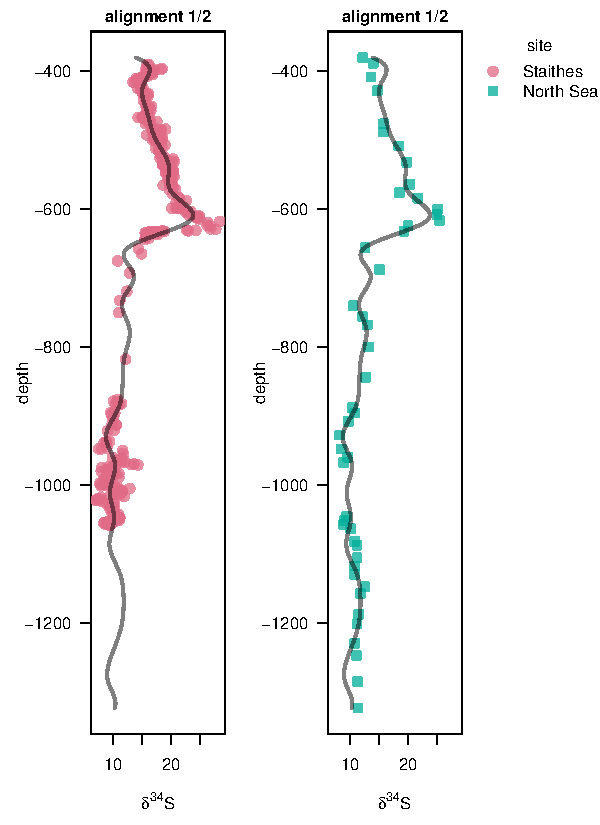
\includegraphics{StratoBayes-Tutorial-1_files/figure-pdf/fig-6-1.pdf}

}

\caption{\label{fig-6}Most likely alignment estimated by the model run.
The North Sea data are plotted at the median reference section depths.}

\end{figure}%

Per default, \texttt{plot()} shows the data from the reference site
(Staithes) along with the shifted section (North Sea) on the depth scale
of the reference section. The heights of the data points from the North
Sea curve are drawn using the iteration that is closest to median
reference section depths (\(50^{th}\) percentile) of a subset of
reference depths (see
\href{https://egusphere.copernicus.org/preprints/2025/egusphere-2025-1355/}{Eichenseer
et al.~in review}), calculated from the posterior draws corresponding to
the most likely alignment (alignment 1/2). In this case, the result
suggests more than one (i.e.~two) possible alignments. The different,
discrete alignments are determined by performing a clustering analysis
on the posterior samples of the model parameters, \(\alpha_{North Sea}\)
and \(\log \gamma_{North Sea}\) in our case. Per default, the first half
of all samples (iterations of the MCMC) are discarded as burn-in, and
are not included in the clustering analysis or in the display of the
results.

Let us visualise the other possible alignments alongside the first:

\begin{Shaded}
\begin{Highlighting}[]
\FunctionTok{par}\NormalTok{(}\AttributeTok{mar =} \FunctionTok{c}\NormalTok{(}\DecValTok{4}\NormalTok{, }\DecValTok{4}\NormalTok{, }\DecValTok{1}\NormalTok{, }\DecValTok{1}\NormalTok{), }\AttributeTok{mfrow =} \FunctionTok{c}\NormalTok{(}\DecValTok{1}\NormalTok{, }\DecValTok{2}\NormalTok{))}
\FunctionTok{plot}\NormalTok{(result, }\AttributeTok{xlab =} \FunctionTok{expression}\NormalTok{(delta}\SpecialCharTok{\^{}}\DecValTok{34}\SpecialCharTok{*}\NormalTok{S), }\AttributeTok{overridePar =} \ConstantTok{FALSE}\NormalTok{, }\AttributeTok{separateSites =}\NormalTok{ F)}
\FunctionTok{plot}\NormalTok{(result, }\AttributeTok{xlab =} \FunctionTok{expression}\NormalTok{(delta}\SpecialCharTok{\^{}}\DecValTok{34}\SpecialCharTok{*}\NormalTok{S), }\AttributeTok{overridePar =} \ConstantTok{FALSE}\NormalTok{, }\AttributeTok{alignment =} \DecValTok{2}\NormalTok{, }\AttributeTok{separateSites =}\NormalTok{ F)}
\end{Highlighting}
\end{Shaded}

\begin{figure}[H]

\centering{

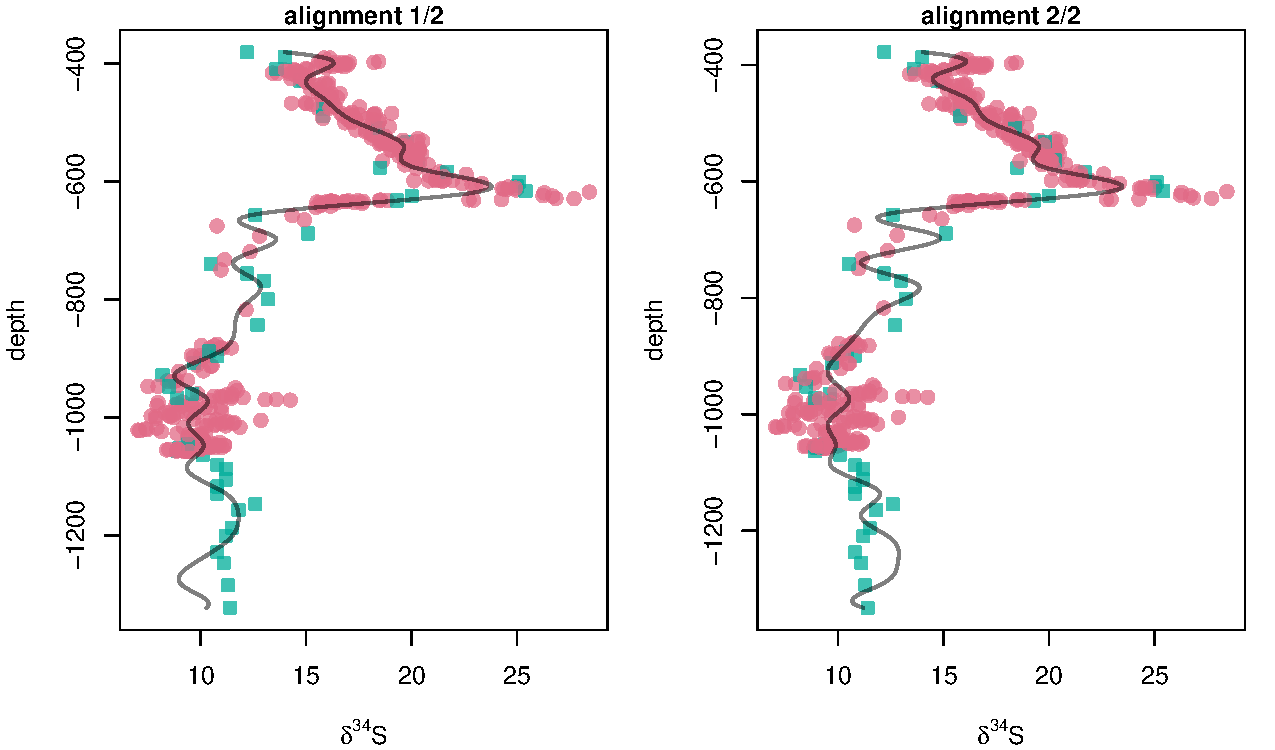
\includegraphics{StratoBayes-Tutorial-1_files/figure-pdf/fig-7-1.pdf}

}

\caption{\label{fig-7}Three distinct alignments found in the posterior
of the model run.}

\end{figure}%

The two alignments don't look very different -- the major peak at -600 m
is always aligned.

\subsection{The parameter estimates}\label{the-parameter-estimates}

To understand why the results suggest these different alignments, we can
inspect the parameter estimates. Visualising the posterior samples in a
histogram works with the \texttt{hist()} function. We want to show both
the \(\alpha_{North Sea}\) and \(\log \gamma_{North Sea}\) parameters,
and colour the parameter values by the alignment they have been
classified in the cluster analysis:

\begin{Shaded}
\begin{Highlighting}[]
\FunctionTok{par}\NormalTok{(}\AttributeTok{mar =} \FunctionTok{c}\NormalTok{(}\DecValTok{4}\NormalTok{, }\DecValTok{4}\NormalTok{, }\FloatTok{0.5}\NormalTok{, }\FloatTok{0.5}\NormalTok{))}
\FunctionTok{hist}\NormalTok{(result, }\AttributeTok{parameters =} \FunctionTok{c}\NormalTok{(}\DecValTok{1}\NormalTok{, }\DecValTok{2}\NormalTok{), }\AttributeTok{colourBy =} \StringTok{"alignment"}\NormalTok{, }\AttributeTok{prior =}\NormalTok{ F)}
\end{Highlighting}
\end{Shaded}

\begin{figure}[H]

\centering{

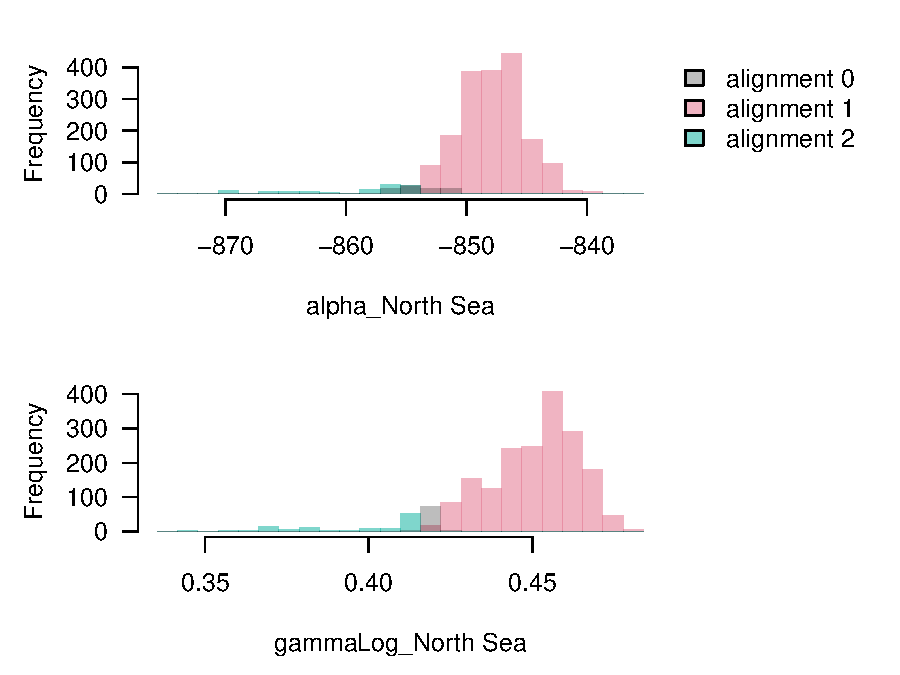
\includegraphics{StratoBayes-Tutorial-1_files/figure-pdf/fig-8-1.pdf}

}

\caption{\label{fig-8}Histograms of the posterior samples of the alpha
and gamma parameter.}

\end{figure}%

Now it is more clear why the results suggest two distinct alignments.
The clustering algorithm has cut the left tail of the distributions, and
a few posterior samples have not been assigned to any cluster
(``alignment 0'').

We can also visualise the parameters in 2D:

\begin{Shaded}
\begin{Highlighting}[]
\FunctionTok{ScatterPlot}\NormalTok{(result, }\AttributeTok{colourBy =} \StringTok{"alignment"}\NormalTok{)}
\end{Highlighting}
\end{Shaded}

\begin{figure}[H]

\centering{

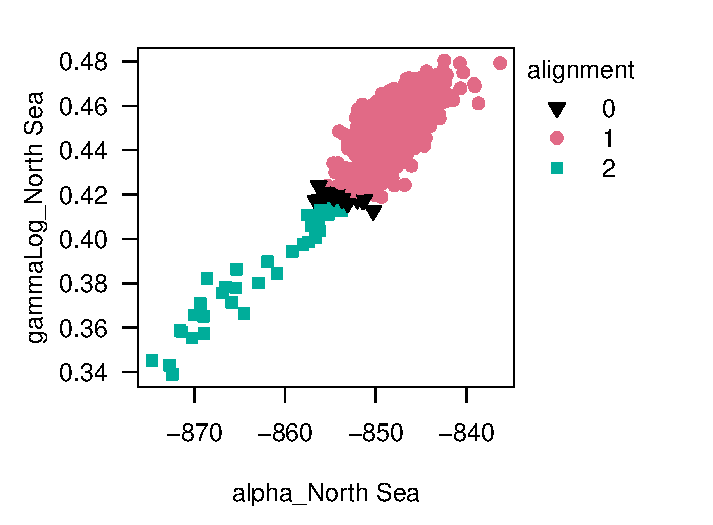
\includegraphics{StratoBayes-Tutorial-1_files/figure-pdf/fig-9-1.pdf}

}

\caption{\label{fig-9}Cross plot of the posterior samples of the alpha
and gamma parameter.}

\end{figure}%

If we are unhappy with the clustering analysis, we could try to change
it. For example, we could use the hierarchical dbscan (``hdbscan'')
method instead of the default protoclust (``proto'') method, using the
\texttt{Cluster()} function:

\begin{Shaded}
\begin{Highlighting}[]
\NormalTok{newClust }\OtherTok{\textless{}{-}} \FunctionTok{Cluster}\NormalTok{(result, }\AttributeTok{clusterMethod =} \StringTok{"hdbscan"}\NormalTok{, }\AttributeTok{minPts =} \DecValTok{10}\NormalTok{)}
\FunctionTok{ScatterPlot}\NormalTok{(result, }\AttributeTok{colourBy =} \StringTok{"alignment"}\NormalTok{, }\AttributeTok{stratCluster =}\NormalTok{ newClust)}
\end{Highlighting}
\end{Shaded}

\begin{figure}[H]

\centering{

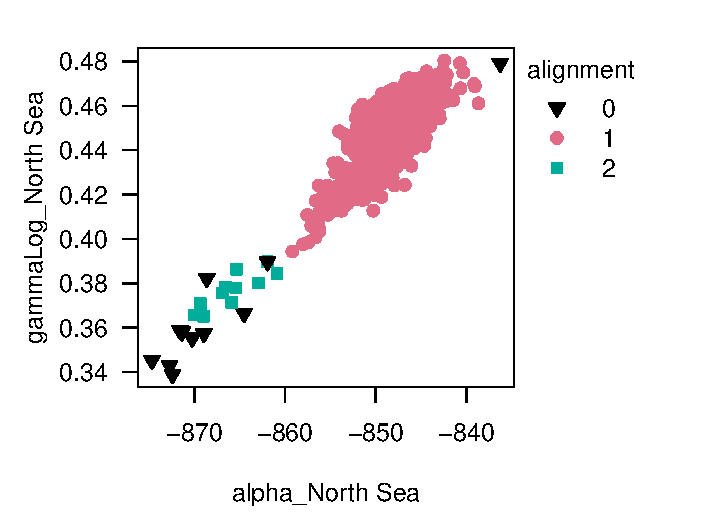
\includegraphics{StratoBayes-Tutorial-1_files/figure-pdf/fig-9b-1.pdf}

}

\caption{\label{fig-9b}Cross plot of the posterior samples of the alpha
and gamma parameter, using hdbscan clustering}

\end{figure}%

This looks like a more natural separation into two clusters.

\subsection{Assessing convergence}\label{assessing-convergence}

An important step in evaluating the model results is to check whether
the chain(s) of our Markov chain Monte Carlo simulation have converged.
Trace plots, in which the posterior samples of model parameters are
shown in the order in which they were obtained, are a great tool for
that:

\begin{Shaded}
\begin{Highlighting}[]
\FunctionTok{par}\NormalTok{(}\AttributeTok{mar =} \FunctionTok{c}\NormalTok{(}\DecValTok{4}\NormalTok{, }\DecValTok{4}\NormalTok{, }\FloatTok{0.5}\NormalTok{, }\FloatTok{0.5}\NormalTok{))}
\FunctionTok{TracePlot}\NormalTok{(result, }\AttributeTok{parameters =} \FunctionTok{c}\NormalTok{(}\DecValTok{1}\NormalTok{, }\DecValTok{2}\NormalTok{))}
\end{Highlighting}
\end{Shaded}

\begin{figure}[H]

\centering{

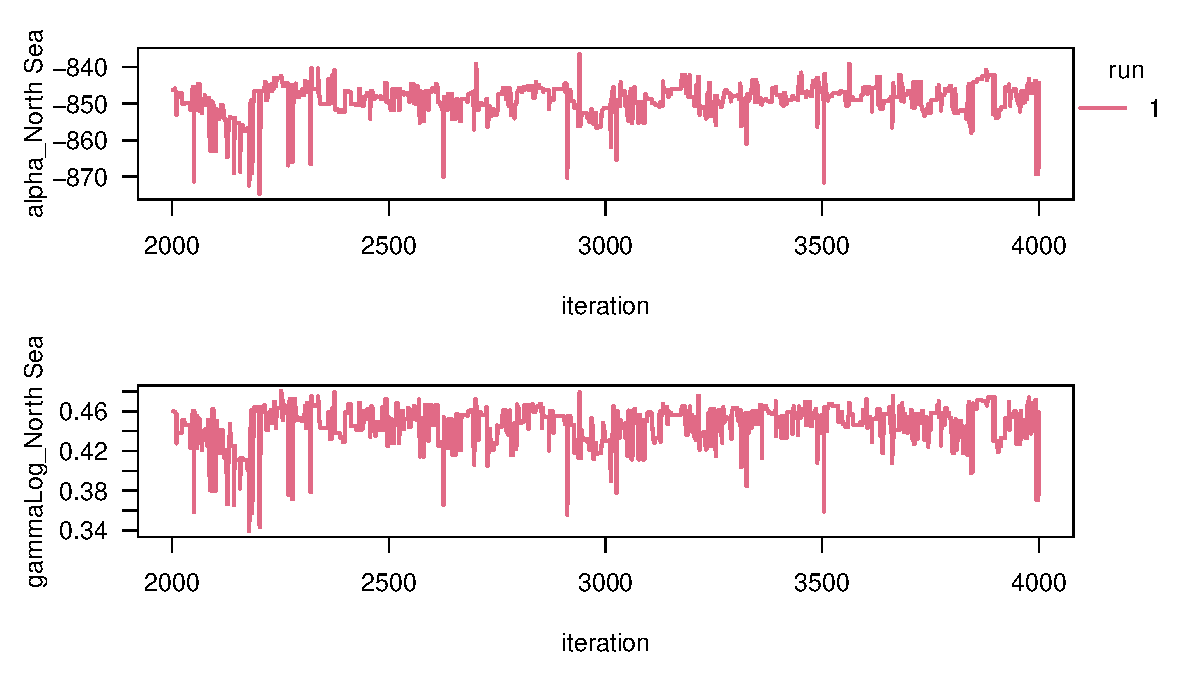
\includegraphics{StratoBayes-Tutorial-1_files/figure-pdf/fig-10-1.pdf}

}

\caption{\label{fig-10}Trace plot showing the posterior samples of the
alpha and gamma parameter in the sequence in which they were obtained
during the MCMC (after burn-in).}

\end{figure}%

Here we can see that the chain looks like it may have converged (the
posterior samples don't seem to shift into new, unexplored areas over
time). There still seems to be a lot of autocorrelation in the chain,
and if we had let the model run for longer, we would probably get
somewhat different estimates for the model parameters and the
probabilities of different alignments.

Another tool to assess convergence is to to look at the posterior
probabilities associated with each of the samples obtained from the
MCMC:

\begin{Shaded}
\begin{Highlighting}[]
\FunctionTok{TracePlot}\NormalTok{(result, }\AttributeTok{parameters =} \StringTok{"posterior"}\NormalTok{)}
\end{Highlighting}
\end{Shaded}

\begin{figure}[H]

\centering{

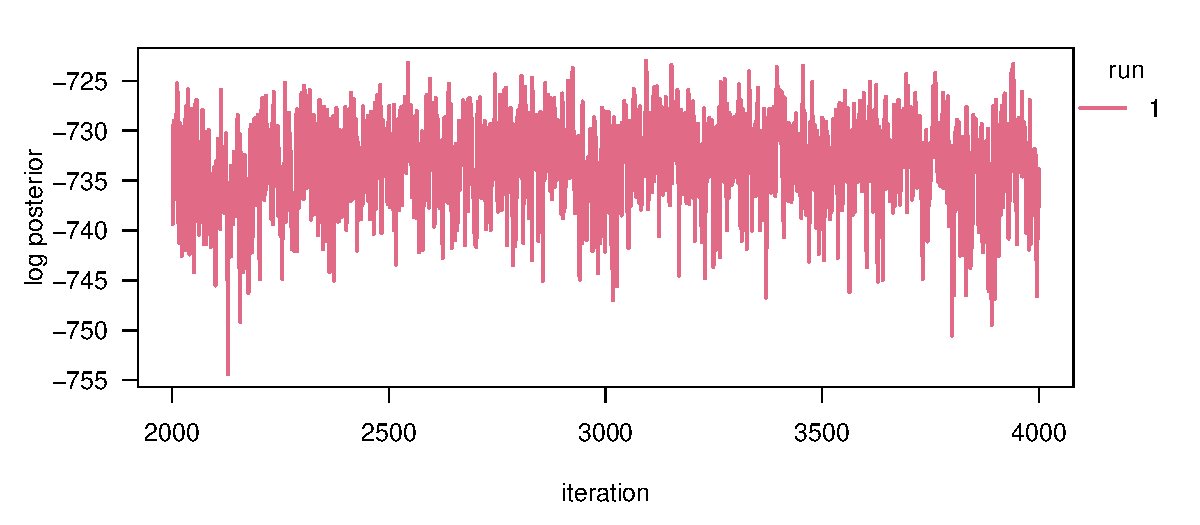
\includegraphics{StratoBayes-Tutorial-1_files/figure-pdf/fig-11-1.pdf}

}

\caption{\label{fig-11}Evolution of the log posterior density during the
MCMC (after burn-in).}

\end{figure}%

The log posterior being relatively stable is a good sign. If it would
increase with increasing iteration number, this would be a tell that the
chain hasn't converged yet.

Ideally, more than one independent model run is conducted. If they all
give a similar answer, that is a good sign.

\subsection{Depths on reference scale}\label{depths-on-reference-scale}

To get the depth in the reference section (Staithes) that correspond to
the shifted depths of the aligned North Sea section, the
\texttt{StratMap()} function can be used. For example, the depths at the
Staithes site that correspond to \(-1900 \, \text{m}\) and
\(-2400 \, \text{m}\) at the North Sea site (\texttt{site\ =\ 2}) can be
computed as follows:

\begin{Shaded}
\begin{Highlighting}[]
\FunctionTok{StratMap}\NormalTok{(result, }\AttributeTok{heights =} \FunctionTok{c}\NormalTok{(}\SpecialCharTok{{-}}\DecValTok{1900}\NormalTok{, }\SpecialCharTok{{-}}\DecValTok{2400}\NormalTok{), }\AttributeTok{site =} \DecValTok{2}\NormalTok{, }\AttributeTok{alignment =} \StringTok{"all"}\NormalTok{)}
\end{Highlighting}
\end{Shaded}

\begin{verbatim}
  height      mean       sd      2.5%       50%     97.5%
1  -1900 -636.8809 2.080428 -640.8139 -636.8918 -633.0691
2  -2400 -956.8522 6.191525 -969.7813 -955.6859 -948.1615
\end{verbatim}

A depth of \(-1900 \, \text{m}\) from the North Sea well corresponds to
a mean depth of \(-637 \, \text{m}\) in the Staithes well. Note that
this depth comes with uncertainty, in this case, the 95\% credible
interval, spanned by the \(0.025\) and the \(0.975\) quantiles ranges
from \(-640.8 \, \text{ to } -633.1 \, \text{m}\). This is quite a low
uncertainty, as the the prominent \(\delta^{34}S_{evap}\) peak allows
for precise alignment.

The uncertainty around the reference depth corresponding to
\(-2400 \, \text{m}\) in the North Sea well is much higher because each
of the two distinct alignments shown earlier results in a different
reference depth for the lower part of the section, and there is
considerable variation also within the alignment clusters.

If we want to just use one alignment to compute the reference depth and
uncertainty, we can specify for example \texttt{alignment\ =\ 1} to use
alignment 1:

\begin{Shaded}
\begin{Highlighting}[]
\FunctionTok{StratMap}\NormalTok{(result, }\AttributeTok{heights =} \FunctionTok{c}\NormalTok{(}\SpecialCharTok{{-}}\DecValTok{1900}\NormalTok{, }\SpecialCharTok{{-}}\DecValTok{2400}\NormalTok{), }\AttributeTok{site =} \DecValTok{2}\NormalTok{, }\AttributeTok{alignment =} \DecValTok{1}\NormalTok{)}
\end{Highlighting}
\end{Shaded}

\begin{verbatim}
  height      mean       sd      2.5%       50%     97.5%
1  -1900 -636.9152 2.101876 -640.8139 -636.9495 -633.0691
2  -2400 -955.4025 3.829975 -963.2279 -955.1406 -948.0990
\end{verbatim}

Here, the uncertainty of the reference depth corresponding to
\(-2400 \, \text{m}\) is much lower.

We can visualise the reference depths corresponding to North Sea depths
by using the \texttt{StratMapPlot()} function:

\begin{Shaded}
\begin{Highlighting}[]
\FunctionTok{StratMapPlot}\NormalTok{(result, }\AttributeTok{alignment =} \StringTok{"all"}\NormalTok{)}
\end{Highlighting}
\end{Shaded}

\begin{figure}[H]

\centering{

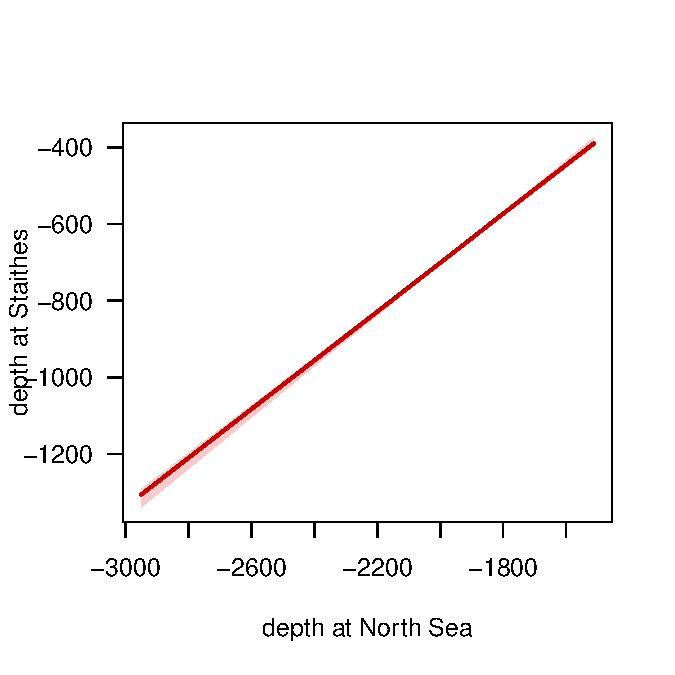
\includegraphics{StratoBayes-Tutorial-1_files/figure-pdf/fig-12-1.pdf}

}

\caption{\label{fig-12}Median depths (line) with 95\% credible intervals
(shading) in the reference section (Staithes) corresponding to depths in
the North Sea section, using all alignments from the posterior (after
burn-in).}

\end{figure}%




\end{document}
